\chapter{Модуль позиционирования}\label{ch:modul}

Вторая половина системы --- маленькая плата с камерой, которая смотрит вниз на ковёр. Мы сначала считали её «позиционным модулем» с неизвестной начинкой. Подключив её к компьютеру по USB, мы убедились, что внутри полноценный компьютер.

\section{Железо}

\begin{itemize}
  \item Чип \textbf{Allwinner V831} (маркировка на кристалле): процессор Cortex-A7 с нейроускорителем. \pr{}
  \item Кнопки \textbf{BOOT} и \textbf{RST}, контакты 5V и GND, два разъёма с линиями TX и RX, USB. \pr{}
  \item Разъём с подписями \textbf{U0TX, U0RX, 5V, GND} ведёт к порту UART0 процессора (в системе модуля \texttt{/dev/ttyS0}). К дрону модуль подключён другим портом (\texttt{ttyS1}), поэтому UART0 свободен для внешних устройств: на него мы подключили зуммер (глава~\ref{ch:pult}). \pr{}
  \item Камера и датчик расстояния \textbf{ToF VI5300}, светодиоды \textbf{WS2812}. \pr{}
\end{itemize}

\begin{figure}[tbp]
\centering
\begin{minipage}[t]{0.485\textwidth}
  \centering
  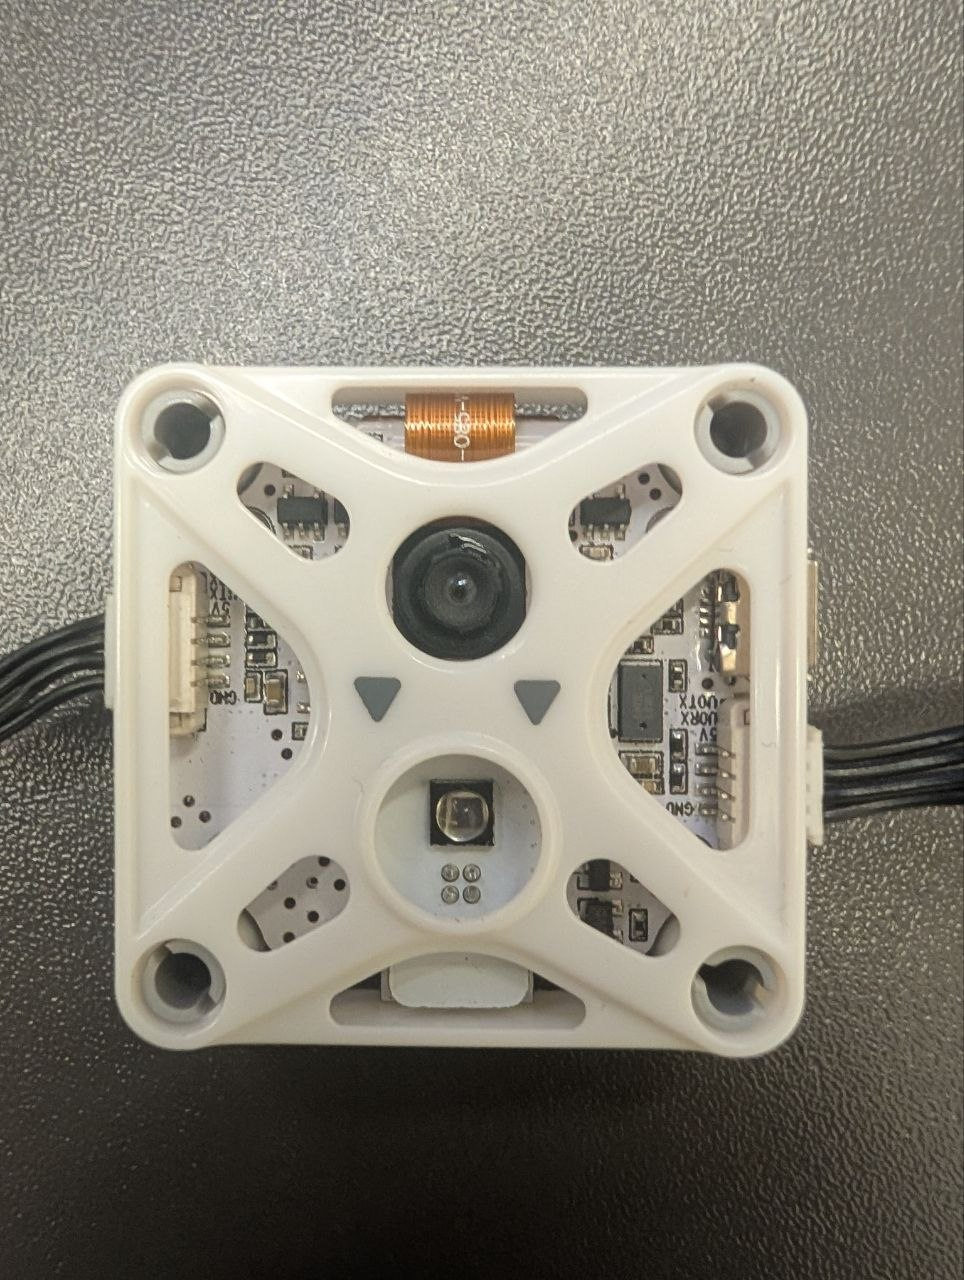
\includegraphics[width=\textwidth]{figures/module_front.jpg}\par\vspace{2pt}
  {\sffamily\small\color{inkgray} (а) со стороны камеры}
\end{minipage}\hfill
\begin{minipage}[t]{0.485\textwidth}
  \centering
  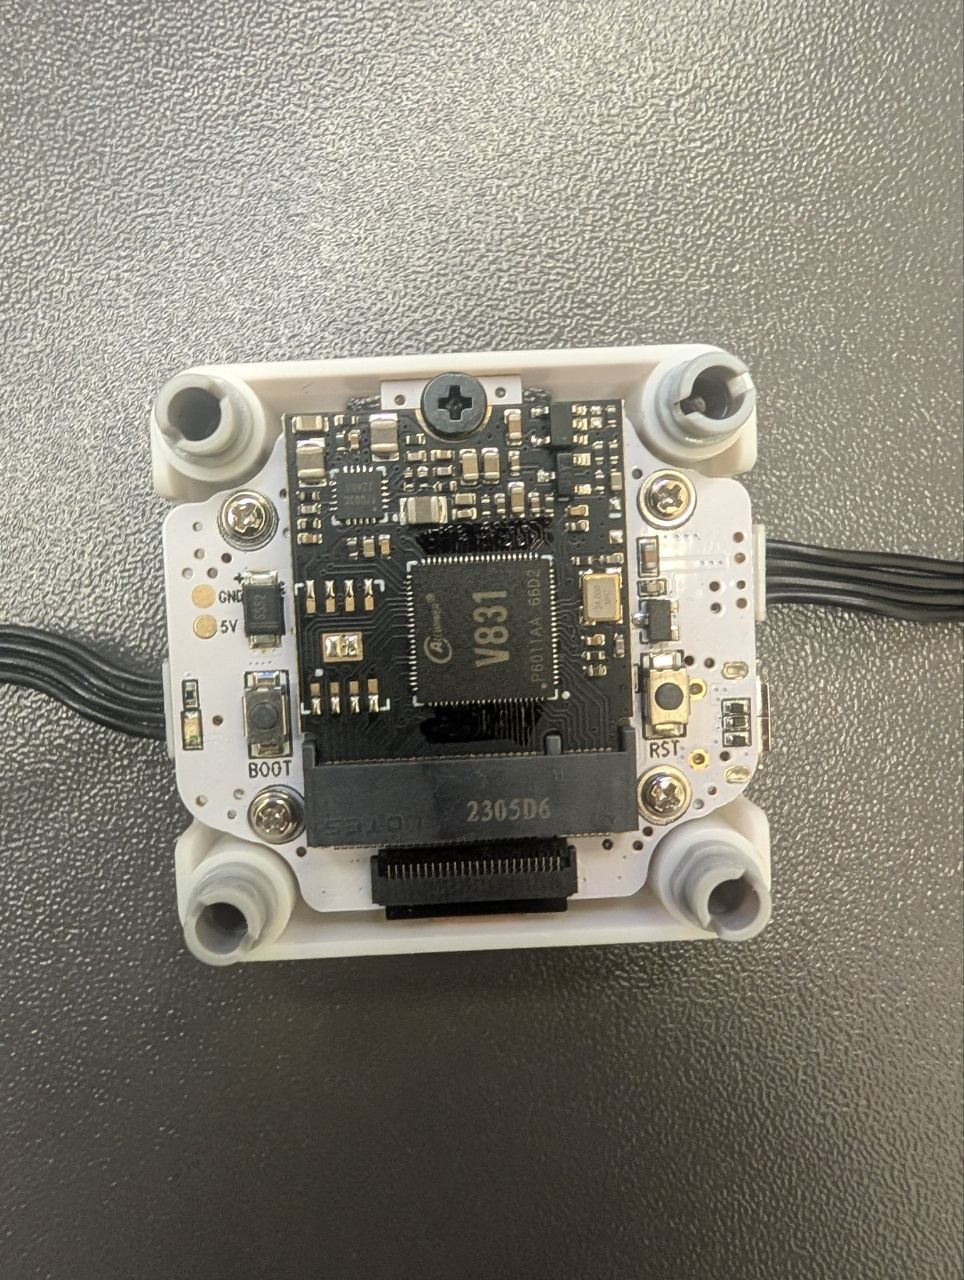
\includegraphics[width=\textwidth]{figures/module_back.jpg}\par\vspace{2pt}
  {\sffamily\small\color{inkgray} (б) со стороны платы}
\end{minipage}
\caption{Модуль позиционирования Wing. Слева: объектив, светодиоды, датчик расстояния (круглое окно снизу), разъёмы с подписями 5V, TX, RX, GND. Справа: чип Allwinner V831, кнопки BOOT и RST, площадки 5V и GND, разъём камеры.}\label{fig:module}
\end{figure}

\section{Операционная система}

Подключённый к компьютеру модуль показывается как устройство \texttt{18D1:0002} (ADB) и как флеш-диск на 50 МБ. Через ADB мы получили оболочку и прочитали систему.

\begin{tabularx}{\textwidth}{@{}p{3.6cm} Y@{}}
\toprule
\hdr{Параметр} & \hdr{Значение} \\ \midrule
Ядро & Linux 4.9.118, дистрибутив OpenWrt, собрано Sipeed, 32-бит ARM. \pr{} \\
Имя узла & \texttt{sipeed}. \pr{} \\
Библиотека C & musl, оболочка BusyBox, есть Python. \pr{} \\
Права доступа & \texttt{root} через ADB. \pr{} \\
Разделы & Корень 254 МБ, \texttt{/mnt/cfg} 69 МБ (программа и настройки), \texttt{/mnt/UDISK} 47 МБ (то, что видно как USB-диск). \pr{} \\ \bottomrule
\end{tabularx}

\section{Программа}

Модулем управляет программа \texttt{app\_ckh831} (всего 14 КБ) и большая библиотека \texttt{libmaix\_ckh831.so} (1,5 МБ), в которой лежит вся работа. Динамические символы библиотеки не вычищены, поэтому мы увидели имена функций. Запускает программу цепочка скриптов: \texttt{S02app} $\to$ \texttt{keep\_app.sh} (следит за процессом) $\to$ \texttt{app\_ckh831}. \pr{}

\begin{zametka}[Откуда взялся детектор]
В библиотеке находится порт \textbf{imlib из OpenMV} --- известной библиотеки компьютерного зрения для маленьких камер. Поиск меток AprilTag (\texttt{apriltag\_detector\_detect}), блобов и цвета --- это функции imlib. Сверху добавлены протокол обмена с дроном, датчик расстояния, светодиоды и графика. \pr{}
\end{zametka}

\section{Какие метки умеет искать модуль}

В библиотеку скомпилированы таблицы пяти семейств: \texttt{tag36h11}, \texttt{tag36h10}, \texttt{tag25h9}, \texttt{tag25h7}, \texttt{tag16h5}. Программа создаёт детектор вызовом \texttt{imlib\_find\_apriltags\_new(0x10, ширина, высота)}. Первый аргумент --- маска семейств, и в нумерации OpenMV значение \texttt{0x10} означает \textbf{только \texttt{tag36h11}}. Семейства ArUco в библиотеке нет. \pr{}

\section{Три режима}

Программа умеет работать в трёх режимах. Номер режима дрон выбирает специальной командой (глава~\ref{ch:uart}).

\begin{tabularx}{\textwidth}{@{}c p{4.2cm} Y@{}}
\toprule
\hdr{№} & \hdr{Режим} & \hdr{Функция в библиотеке} \\ \midrule
0 & Поиск меток AprilTag & \texttt{get\_imlib\_find\_apriltag\_app} \\
1 & Поиск блобов (цветных пятен, вероятно, для линии) & \texttt{get\_imlib\_find\_blobs\_app} \\
2 & Поиск цвета & \texttt{get\_imlib\_find\_color} \\ \bottomrule
\end{tabularx}

\vspace{4pt}
\pr{} Порядок взят из таблицы перемещений самой библиотеки. Выбранный режим программа запоминает в JSON-конфигурации.

\section{Датчик расстояния и светодиоды}

Модуль меряет расстояние до пола датчиком ToF VI5300 по шине I\textsuperscript{2}C. Это расстояние уходит дрону в каждом кадре (раздел~\ref{sec:frame}). Светодиоды WS2812 управляются командами дрона; у таких светодиодов порядок цветов \emph{зелёный, красный, синий}, и ровно такой же порядок мы нашли в команде приложения \texttt{set\_ledRGB}. \pr{}

\section{Что видит камера}

Чтобы увидеть то же, что видит модуль, мы остановили на нём программу детектора и сняли серию кадров стандартным Python-модулем \texttt{maix.camera}. Кадр имеет размер 320$\times$240 (штатная программа работает с уменьшенным кадром 160$\times$120). Модуль держали под углом около 45\textdegree{} над листом с меткой 13. \pr{}

\begin{figure}[tbp]
\centering
\fbox{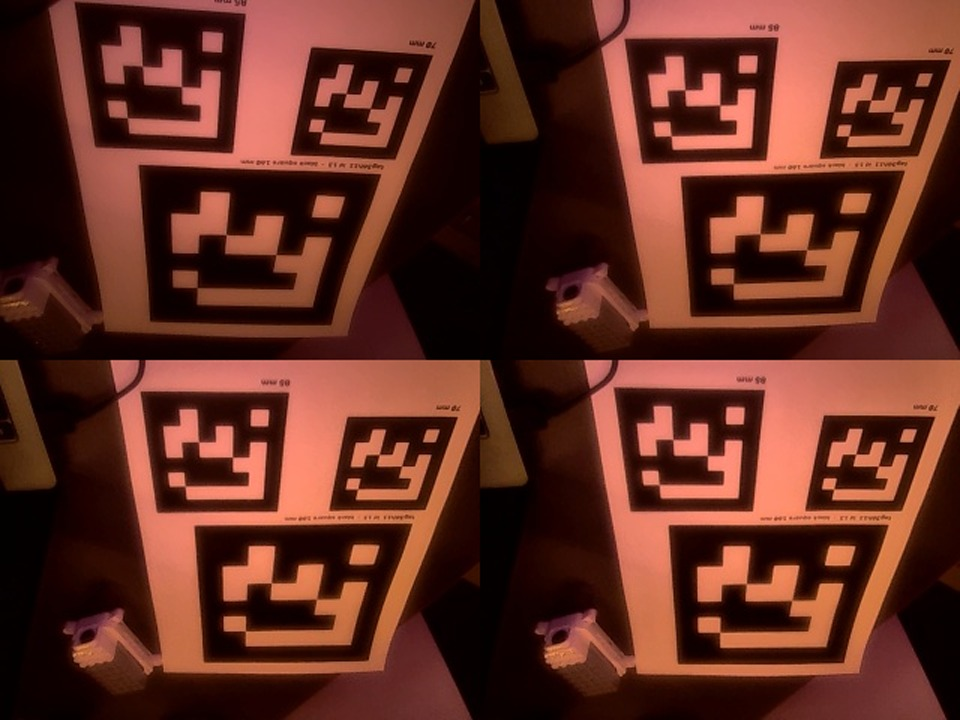
\includegraphics[width=\dimexpr0.92\textwidth-2\fboxsep-2\fboxrule\relax]{figures/module_camera.jpg}}
\caption{Четыре кадра с камеры модуля (под углом около 45\textdegree). Лист в кадре повёрнут вверх ногами: на нём три одинаковые метки 13 размером 160, 85 и 70 мм. Розовый оттенок даёт собственная подсветка модуля.}\label{fig:modcam}
\end{figure}

Отсюда видно несколько вещей:
\begin{itemize}
  \item В кадре сразу несколько меток (это три размера на одном листе). Штатная программа выбирает ту, что ближе к центру кадра.
  \item Метки хорошо читаются даже под углом. OpenCV на тех же кадрах нашёл номер 13 на всех десяти снимках (по две--три метки на кадре).
  \item Цвет с розовым оттенком: подсветка тёплая, камера без инфракрасного фильтра или с узкой полосой. \vyv{}
  \item Лист был напечатан тремя размерами сразу, поэтому по этим кадрам нельзя сказать, какая именно метка использовалась в расчёте, и подтвердить размер около 100 мм.
\end{itemize}

\section{Подсветка: почему метка видна в темноте}

Владелец проверил: модуль опознаёт метку в полной темноте. Объяснение нашлось в самом модуле. В системе включены \textbf{четыре канала ШИМ} (период 10 мс, то есть 100 Гц) со скважностью \textbf{97,5\,\%}. Программа инициализирует ШИМ при старте и снова задаёт его при входе в режим меток, а команды дрона 4 и 6 тоже меняют ШИМ. \pr{}

Вывод (\vyv{}): ШИМ управляет собственной светодиодной подсветкой модуля, которая светит почти на полную яркость. На фото платы по углам лицевой стороны виден ряд малых компонентов, похожих на ключи подсветки, но это предположение.

\begin{zametka}[Для своей камеры]
Освещение входит в систему. Камере, которая сама не светит, понадобится столько же света (или инфракрасная подсветка), иначе метки в темноте не распознаются. Яркостью модуля можно управлять командами дрона.
\end{zametka}

\section{Что внутри образа флеша}

Мы сняли побитовый образ всего флеша модуля (482 МБ) и разобрали его. Вывод оказался простым: \textbf{под программой производителя лежит готовый образ Sipeed MaixPy3}. \pr{}

\begin{tabularx}{\textwidth}{@{}p{3.1cm} Y@{}}
\toprule
\hdr{Раздел} & \hdr{Что внутри} \\ \midrule
\texttt{env}, \texttt{boot} & Переменные загрузчика и ядро (256 КБ и 4 МБ). \\
\texttt{cfg} (75 МБ) & Только программа производителя: каталог \texttt{firmware/maix\_dist}. \\
\texttt{rootfs} (256 МБ) & Стандартный MaixPy3 0.5.4: Linux, Python 3.8, \texttt{numpy}, \texttt{pyserial}, \texttt{Pillow}, модуль \texttt{maix} (камера, ШИМ, GPIO, UART), модели нейросетей, библиотеки OpenCV 4.1 для C++. \\
\texttt{swap}, \texttt{UDISK} & Раздел подкачки и USB-диск (FAT). \\ \bottomrule
\end{tabularx}

\vspace{4pt}
Из этого следует несколько практических вещей:
\begin{itemize}
  \item В Python уже есть \texttt{find\_apriltags} (тот же код imlib), а также поиск QR-кодов, линий, кругов и прямоугольников.
  \item Библиотека OpenCV \texttt{aruco} есть, но только для C++. Привязки \texttt{cv2} для Python нет.
  \item Серийный номер USB \texttt{20080411} и производитель \texttt{MaixPy3} задаются скриптом \texttt{S12usb}: поэтому он совпадает у модуля и у дрона (общий для платформы).
  \item Скрипт запуска \texttt{S02app} запускает \texttt{/root/main.py} (файл на USB-диске модуля) вместо штатной программы. Это самый короткий путь к своей камере (глава~\ref{ch:svoya}). \vyv{}
\end{itemize}

\subsection*{Калибровка камеры}

Параметры камеры лежат в самой программе как числа: кадр \textbf{160$\times$120} пикселей, центр (80, 60), фокусное расстояние около \textbf{112,5 и 113,8} пикселя по осям. Из найденных меток выбирается та, что ближе к центру кадра. Выходные числа получаются так: положение метки умножается на $-100$, угол поворота в радианах умножается на 572, то есть получаются десятые доли градуса. \pr{}

По живым кадрам (расстояние метки 296--329 при ToF 287--311 мм) штатная программа ведёт себя так, как если бы метка имела сторону около 100 мм. Это вывод, а не прочитанное число. \vyv{}

\section{Как обновляется программа}

Самое неожиданное в модуле --- способ обновления. На USB-диске модуля лежат три файла: \texttt{maix\_dist.sha256sum}, \texttt{V1.0.3} и \texttt{color\_config.json}. Если рядом положить папку \texttt{maix\_dist} с новой программой, то при следующем запуске скрипт \texttt{S02app} делает следующее. \pr{}

\begin{enumerate}
  \item Видит файл \texttt{maix\_dist/maix\_dist.sha256sum}.
  \item Копирует папку \texttt{maix\_dist} во внутреннюю память (\texttt{/mnt/cfg/firmware}).
  \item Удаляет её с диска.
  \item Перезагружает модуль.
\end{enumerate}

\begin{figure}[tbp]
\centering
\begin{tikzpicture}[
  st/.style={draw=rule, fill=paper, rounded corners=3pt, minimum height=11mm, minimum width=33mm, align=center, font=\sffamily\small},
  ar/.style={-{Stealth[length=2.4mm]}, color=accentdark, line width=0.8pt}
]
\node[st] (a) {USB-диск\\\texttt{maix\_dist}};
\node[st, right=12mm of a] (b) {старт:\\\texttt{S02app}};
\node[st, right=12mm of b] (c) {копия в\\\texttt{/mnt/cfg}};
\node[st, right=12mm of c] (d) {перезапуск};
\draw[ar] (a)--(b); \draw[ar] (b)--(c); \draw[ar] (c)--(d);
\end{tikzpicture}
\caption{Обновление программы модуля через USB-диск.}\label{fig:upd}
\end{figure}

\begin{vnimanie}[Сброс при ошибке]
Если новая программа падает и запускается четыре раза подряд, сторожевой скрипт \texttt{keep\_app.sh} вызывает \texttt{factory.sh}, то есть сбрасывает модуль. Это защита, но и риск: перед любыми изменениями нужно иметь полную копию. Мы её сняли (103 файла, около 30 МБ). \pr{}
\end{vnimanie}
